\documentclass[margin=.2cm]{standalone}

\usepackage{tikz}
\usetikzlibrary{calc,arrows}

  %% We define the name of each number
  \newcommand\savename[2]{\expandafter\xdef\csname name#1\endcsname{#2}}
  \newcommand\getname[1]{\csname name#1\endcsname}


\begin{document}

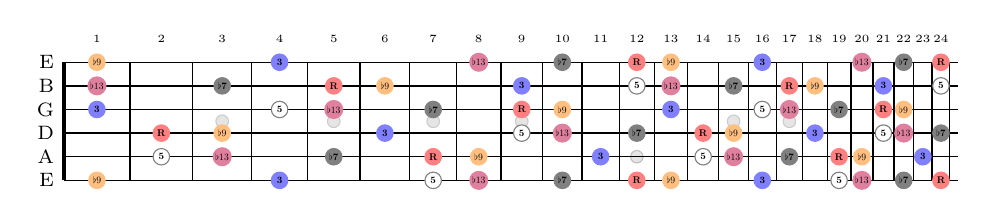
\begin{tikzpicture}[
    ynode/.style={draw=black!50,circle,fill=black!50,scale=.35,inner sep=1pt,minimum size=1.7em}, rnode/.style={draw=red!50,circle,fill=red!50,scale=.35,inner sep=1pt,minimum size=1.7em},
    thirdnode/.style={draw=blue!50,circle,fill=blue!50,scale=.35,inner sep=1pt,minimum size=1.7em},
    fifthnode/.style={draw=black!50,circle,fill=white!50,scale=.35,inner sep=1pt,minimum size=1.7em},
    seventhnode/.style={draw=black!50,circle,fill=black!50,scale=.35,inner sep=1pt,minimum size=1.7em},
    ninthnode/.style={draw=orange!50,circle,fill=orange!50,scale=.35,inner sep=1pt,minimum size=1.7em},
    thirteenthnode/.style={draw=purple!50,circle,fill=purple!50,scale=.35,inner sep=1pt,minimum size=1.7em}]

  %%%% Draw the base and set coordinates %%%%
  \begin{scope}[xscale=-15,yscale=.3,line width=.5]

    \xdef\x{1}
    %% Left line
    \draw[line width=1.5] (1,1) -- (1,6);
    \foreach \fret in {1,...,24}{
      %% Set coordinate for each string
      \foreach \str in {1,...,6}{
        \coordinate (\str-\fret) at (0.97193715634*\x,\str);
      }
      %% Set coordinate for the text above
      \coordinate (Top-\fret) at (0.97193715634*\x,7);
      %% Compute the position of the fret
      \pgfmathsetmacro\x{\x * 0.94387431268}
      \xdef\x{\x}
      %% Draw the fret
      \draw (\x,1) -- (\x,6);
    }

    %% Draw each string
    \foreach \str in {1,...,6}{
      \draw (1,\str) -- (0.97153194115*\x,\str);
      \coordinate (start\str) at (1,\str);
    }
  \end{scope}

  %% Draw the mark on the guitare
  \foreach \f in {3,5,7,9,15,17}{
    \draw[black!20,fill=black!10] ($(3-\f)!.5!(4-\f)$) circle (.08);
  }
  \draw[opacity=.20,fill,fill opacity=.10] (2-12) circle (.08) (5-12) circle (.08);
  \foreach \n/\t in {1/A,2/A$\sharp$,3/B,4/C,5/C$\sharp$,6/D,7/D$\sharp$,8/E,9/F,10/F$\sharp$,11/G,0/G$\sharp$}{
    \savename{\n}{\t}
  }

  %% Boucle on the string and the first note (given its number)
  \foreach \str/\note in {1/8,2/1,3/6,4/11,5/3,6/8}{
    \node[anchor=east] at (start\str) {\scriptsize\getname{\note}};
  }
  \foreach \str/\fret in {1/12,1/24,2/7,2/19,3/2,3/14,4/9,4/21,5/5,5/17,6/12,6/24}{\node[rnode] at (\str-\fret) {\textbf{R}};}
  \foreach \str/\fret in{1/4,1/16,2/11,2/23,3/6,3/18,4/1,4/13,5/9,5/21,6/4,6/16}{\node[thirdnode] at(\str-\fret) {\textbf{3}};}
  \foreach \str/\fret in{1/7,1/19,2/2,2/14,3/9,3/21,4/4,4/16,5/12,5/24,6/8,6/20}{\node[fifthnode] at(\str-\fret) {\textbf{5}};}
  \foreach \str/\fret in{1/10,1/22,2/5,2/17,3/12,3/24,4/7,4/19,5/3,5/15,6/10,6/22}{\node[seventhnode] at(\str-\fret) {\textbf{$\flat$7}};}
  \foreach \str/\fret in{1/1,1/13,2/8,2/20,3/3,3/15,4/10,4/22,5/6,5/18,6/1,6/13}{\node[ninthnode] at(\str-\fret) {\textbf{$\flat$}9};}
  \foreach \str/\fret in{1/8,1/20,2/3,2/15,3/10,3/22,4/5,4/17,5/1,5/13,6/8,6/20}{\node[thirteenthnode] at(\str-\fret) {\textbf{$\flat$}13};}
  
  
  %% Number above each space
  \foreach \fret in {1,...,24}{
    \node[scale=.8] at (Top-\fret) {\tiny \fret};
  }

\end{tikzpicture}

\end{document}